
%%%%%%%%%%%%%%%%%%%%%%% file typeinst.tex %%%%%%%%%%%%%%%%%%%%%%%%%
%
% This is the LaTeX source for the instructions to authors using
% the LaTeX document class 'llncs.cls' for contributions to
% the Lecture Notes in Computer Sciences series.
% http://www.springer.com/lncs       Springer Heidelberg 2006/05/04
%
% It may be used as a template for your own input - copy it
% to a new file with a new name and use it as the basis
% for your article.
%
% NB: the document class 'llncs' has its own and detailed documentation, see
% ftp://ftp.springer.de/data/pubftp/pub/tex/latex/llncs/latex2e/llncsdoc.pdf
%
%%%%%%%%%%%%%%%%%%%%%%%%%%%%%%%%%%%%%%%%%%%%%%%%%%%%%%%%%%%%%%%%%%%


\documentclass[runningheads,a4paper]{llncs}

\setcounter{tocdepth}{3}
\usepackage{graphicx}
% For citations
\usepackage{natbib}
\usepackage{amsmath,amsfonts,amscd,amssymb}
\usepackage{dsfont}
\renewcommand{\vec}[1]{\mathbf{#1}}
\usepackage{hyperref}
\DeclareMathOperator*{\argmax}{argmax}
\DeclareMathOperator*{\argmin}{argmin}
\DeclareMathOperator*{\Corr}{Corr}
\newcommand{\R}{\mathds{R}}
\usepackage{multicol}
\usepackage{multirow}
\usepackage{pbox}
\usepackage{url}
\urldef{\mailsa}\path|{felix.biessmann,|
\newcommand{\keywords}[1]{\par\addvspace\baselineskip
\noindent\keywordname\enspace\ignorespaces#1}

\begin{document}

\mainmatter  % start of an individual contribution

% first the title is needed
\title{Automating Political Bias Prediction}

% a short form should be given in case it is too long for the running head
\titlerunning{Political Bias Prediction}

% the name(s) of the author(s) follow(s) next
%
% NB: Chinese authors should write their first names(s) in front of
% their surnames. This ensures that the names appear correctly in
% the running heads and the author index.
%
\author{
%Felix Bie\ss{}mann%
\thanks{}
%
\authorrunning{Political Bias Prediction}}
% (feature abused for this document to repeat the title also on left hand pages)

% the affiliations are given next; don't give your e-mail address
% unless you accept that it will be published
%\institute{
%\mailsa\\
%\mailsb\\
%\mailsc\\
%\url{http://www.springer.com/lncs}}

%
% NB: a more complex sample for affiliations and the mapping to the
% corresponding authors can be found in the file "llncs.dem"
% (search for the string "\mainmatter" where a contribution starts).
% "llncs.dem" accompanies the document class "llncs.cls".
%

\toctitle{Political Bias Prediction}
\tocauthor{}
\maketitle

\begin{abstract} 
Every day media generate large amounts of text. Getting an unbiased view on what media report on requires an unbiased and heterogenous sample of media content. Assistive technology for estimating the political bias of texts can be helpful in this context. In this study a simple statistical learning approach is presented that can be used to predict political bias from text. Standard text features extracted from political texts are used to train classifiers that predict political bias in terms of a) party affiliation and b) in terms of political views. Results indicate that political bias prediction is possible with well above chance accuracy. The results are further validated by relating discriminative text features to the political orientation of a party. Moreover the results demonstrate that sentiment appears to be a very discriminative feature: Political power of an author strongly correlates with positive sentiment of a text. To highlight some potential use cases a web application shows how the model can be used for texts for which the political bias is not clear such as news articles.
\end{abstract} 

\section{Introduction}
\label{sec:intro}
%
Modern media generate a large amount of content at an ever increasing rate. Keeping an unbiased view on what media report on requires to understand the political bias of texts. In many cases it is obvious which political bias an author has. In other cases some expertise is required to judge the political bias of a text. 
%
When dealing with large amounts of text however there are simply not enough experts to examine all possible sources and publications. Assistive technology can help in this context to try and obtain a more unbiased sample of information. 

Ideally one would choose for each topic a sample of reports from the entire political spectrum in order to form an unbiased opinion. But ordering and assigning media content with respect to the political spectrum at scale requires automated prediction of political bias. The aim of this study is to provide some empirical evidence indicating that political bias prediction is possible with well above chance accuracy. \\


Automated predictions of political bias can be problematic for ethical reasons. One trusts political experts, as they will take responsibility for what they say about a text, and they can explain their decisions. This is a key difference to many statistical learning approaches. Not only is the responsibility question not entirely clear, it can also be difficult to interpret some of the decisions. In order to validate the predictions of the models we devise two strategies that allow for better interpretations of the models. First we are looking at univariate measures of how discriminative the features are that the model uses. This somewhat allows to relate the political texts to the kind of information that political experts use, too. Second we use sentiment analysis to investigate whether this aspect of language also has discriminatory power. \\


In the following \autoref{sec:data} gives an overview of data acquisition and preprocessing, \autoref{sec:model} presents the model, in \autoref{sec:results} the results are discussed and \autoref{sec:conclusion} concludes with some interpretations of the results and future research directions. 

\section{Data Sets and Feature Extraction}\label{sec:data}
%
We used publicly available data sets of german political texts and standard libraries for processing the text. The following sections describe the details of data acquisition and feature extraction. 

\subsection{Data}
We obtained annotated political text data from sources a) the discussions and speeches held in the german parliament ({\em Bundestag}) and b) all manifesto texts from parties running for election in the german parliament in the current 18th and the last, 17th, legislation period.

\paragraph{Parliament discussion data} Parliament texts are annotated with the respective party label, which we take here as a proxy of political bias. The texts of parliament protocols are available through the website of the german bundestag\footnote{\url{https://www.bundestag.de/protokolle}}, we used an open source API to that data to query the data in cleaned and structured format\footnote{\url{https://github.com/bundestag}}. This API returns for each speech the speaker and its party affiliation. In total we obtained 22784 speeches for the 17th legislative period and 11317 speeches for the 18th period, queried until March 2016. 

\paragraph{Party manifesto data}
For party manifestos we also use an openly accessible API provided by the Wissenschaftszentrum Berlin (WZB). The API is released as part of the {\em Manifestoproject} \cite{manifesto}. The data released in this project comprises the complete manifestos for each party that ran for election enriched with annotations by political experts. Each sentence (in some cases also parts of sentences) are labels with one of 56 political labels. Examples of these labels are {\em pro/contra protectionism, decentralism, centralism, pro/contra welfare, ...}. The set of labels was developed by political scientists at the WZB and released for public use. We obtained all manifestos of parties that were running for election in this and the last legislative period. In total this resulted in 29451 political statements that had two types of labels, for one we stored the party affiliation of each political statement. This party affiliation label was used to evaluate the party evaluation classifiers trained on the parliament speeches. For this purpose we constrained the data to only those parties that were elected into the parliament. Next to the party affiliation we were mainly interested in the political view labels annotated by human experts. For the analyses based on political view labels we considered all parties, also those that did not make it into the parliament. 

\subsection{Bag-of-Words Vectorization}\label{sec:bow-vectorization}
For each semantic unit, in the case of parliament discussions this were the speeches\footnote{Often speeches were interrupted; in this case each uninterrupted part of a speech was considered a semantic unit.} in the case of the party manifesto data semantic units were the sentences or sentence parts associated with one of the 56 political view labels. Strings of each semantic unit were tokenized and transformed into bag-of-word vectors as implemented in scikit-learn \cite{scikit-learn}. The general idea of bag-of-words vectors is to simply count occurences of words (or word sequences, also called {\em n-grams}) for each data point (usually documents, here parliament speeches). So the text of each speech is transformed into a vector $\vec{x}\in\mathds{R}^d$, were $d$ is the size of our dictionary; the $w$th entry of $\vec{x}$ contains the (normalized) count of the $w$th word (or sequence of words) in our dictionary. We tried several options for vectorizing the speeches, including term-frequency-inverse-document-frequency normalisation using n-gram patterns up to size $n=3$ and several cutoffs for discarding too frequent and too infrequent words. All of these hyperparameters were subjected to hyperparameter optimization as explained in \autoref{sec:crossvalidation}. 


\section{Classification Model and Training Procedure}\label{sec:model}

We used a multinomial logistic regression model in order to classify bag-of-words feature vectors $\vec{x}\in\R^d$, where $d$ is the size of the bag-of-words dictionary. Let $y\in\{1,2,\dots,K\}$ be the true party label, where $K$ is the total number of parties in the parliament and $\vec{W}=[\vec{w}_1,\dots,\vec{w}_K]\in\R^{d\times K}$ be the concatenation of the weight vectors $\vec{w}_k$ associated with the $k$th party then 
\begin{eqnarray}\label{eq:logreg_multiclass}
p(y=k|\vec{x},\vec{W}) = &\frac{e^{z_k}}{\sum_{j=1}^K e^{z_j}} \qquad \textrm{with }  z_k=&\vec{w}_k^{\top}\vec{x} \\\nonumber
\end{eqnarray}
%
We estimated $\vec{W}$ using quasi-newton gradient descent as packaged in the scikit-learn toolbox. The optimization function was obtained by adding a penalization term to the negative log-likelihood of the multinomial logistic regression objective and the optimization hence found the $\vec{W}$ that minimized
\begin{equation}\label{eq:objective}
L(\vec{W}, \vec{x}, \gamma) = - \log{\frac{e^{z_k}}{\sum_{j=1}^K e^{z_j}}}+ \gamma \| \vec{W} \|_{F}
\end{equation}
Where $\|~\|_F$ denotes the Frobenius Norm and $\gamma$ is a regularization parameter controlling the complexity of the model. 
 We optimized the regularization parameter on a log-scaled grid from $10^{-4,\dots,4}$ and the regularization constant was adopted to reflect asymmetric class frequency distributions. The performance of the model was optimized using the classification accuracy, but we also report all other standard measures, precision ($TP / (FP + TP$), recall ($TP / (TP + FN)$) and f1-score ($2\times (Prec. \times Rec) / (Prec + Rec.)$). 

We considered three different classification problems: 1) classification of party affiliation (5 class problem for the 17th legislation period, 4 class problem for the 18th legislation period), 2) classification of government membership (binary problem) and 3) classification of political views as expressed by the political codes of the manifestoproject (56 class problem). For each of first two problems, party affiliation and government membership prediction, we trained classifiers on the parliament speeches. For the third problem we trained only on the manifesto data as only for those the political view labels were available. 

\subsection{Optimisation of Model Parameters}\label{sec:crossvalidation}
The model pipeline contained a number of {\em hyperparameters} that we did not want to tune by hand. 
We first split the training data into a training data set and a test data set for optimizing the hyperparameters, the test data for hyperparameter optimization was 10\% of the entire training data. Hyperparameters were optimized using grid search: For each setting of hyperparameters the entire pipeline was trained and evaluated on the test set. For the best setting of all hyperparameters, we trained the pipeline again on all training data and evaluated it on the evaluation set. Evaluation data was never used for training the models. For party affiliation prediction and government membership prediction the training and test set were 90\% and 10\%, respectively, of all data in a legislative period. Evaluation data were the texts from party manifestos. For the political view prediction setting we first split all labeled manifesto sentences in both legislative periods into a training/test and evaluation set of 90\% (train/test) and 10\% (evaluation), then we split the train/test part again with a 90\%/10\% ratio for training/testing of the hyperparameters. 

\subsection{Sentiment analysis}\label{sec:sentiment_analysis_methods}
We used a publicly available key word list to extract sentiments from the text subjected to classification \cite{remquahey2010}. The sentiment index used for attributing positive or negative sentiment to a text was computed  as the Pearson correlation coefficient between bag-of-word vectors $\vec{x}\in\R^d$ and sentiment vector $\vec{s}\in\R^d$ which was constructed by simply taking the values from the sentiment dictionary. 

\subsection{Analysing bag-of-words features}
In order to get  better picture of which features contribute to the classification we computed correlation coefficients between each word and each party. Often linear models are interpreted by just looking at the weights of the model. Note that due to the fact that the features are obtained from real data and thus correlated we cannot inspect the model by interpreting the coefficients of $\vec{W}$; for an in-depth discussion of this problem see e.g. \cite{Haufe2013}. The words corresponding to the top positive and negative correlations are shown in section \autoref{sec:word_party_correlations}.

\section{Results}\label{sec:results}

The following sections provide an overview of the results for both types of political bias prediction tasks, party affiliation and political view. Some interpretations of discriminative features are given one section will highlight a finding on the correlation of political power and positive sentiment of political texts. 

\subsection{Predicting political party affiliation}

% Confusion matrix
\begin{table}[t]\label{tab:conf_mat_four_class}
\begin{tabular}{lccccccc}
&&& \multicolumn{5}{c}{Predicted Class}\\
&&& cducsu & fdp& gruene& linke& spd\\
\multirow{5}{*}{\rotatebox{90}{\pbox{3cm}{\centering True Class}}}& &cducsu &1186 &289& 178& 198& 179\\
&&fdp &882& 658& 236& 329& 214\\
&&gruene &1174& 404& 764& 941& 464\\
&&linke &388& 92& 214& 806& 201\\
&&spd &999& 268& 240& 398& 373\\
 \multicolumn{8}{c}{\bf 17th Bundestag}\\
\end{tabular}
\quad
\begin{tabular}{lcccccc}
&&& \multicolumn{4}{c}{Predicted Class}\\
&&& cducsu & gruene& linke& spd\\
\multirow{4}{*}{\rotatebox{90}{\pbox{3cm}{\centering True Class}}}&&cducsu&1912& 156& 331& 584\\
&&gruene&2092& 827& 1311& 1444\\
&&linke&596& 186& 1216& 557\\
&&spd&1284& 226& 563& 916\\
 \multicolumn{7}{c}{\bf 18th Bundestag}\\
\end{tabular}
\caption{\label{tab:confusion} Confusion matrices for predictions on evaluation data (party manifestos) for classifiers trained on parliament speeches for the 17th legislative period (left) and 18th legislative period (right); the most prominent effect is the high likelihood for a party to be taken as the strongest, governing party, cdu/csu. In particular the green party suffers from this effect: when trained on the speeches in the 18th Bundestag, 2092 statements out of the green party's manifesto were classified as belonging to the cducsu party. This can be interpreted as a change in policies of the conservative party cdu/csu towards the policies of the green party.}
\end{table}

\begin{table}[t]
\begin{center}
\begin{tabular}{lcccccccc}
& \multicolumn{4}{c}{\bf Held-out parliament speeches} & \multicolumn{4}{c}{\bf Party Manifestos}\\
    &         precision    &recall &  f1-score  & N    &         precision    &recall &  f1-score  & N\\
\hline \hline
       cducsu   &    0.62  &    0.81  &    0.70  &     706&0.26    &  0.58   &   0.36    &  2030\\
        fdp    &   0.70   &   0.37  &    0.49    &   331&0.38   &   0.28    &  0.33   &   2319\\
     gruene &      0.59  &    0.40   &   0.48   &    298&0.47  &    0.20   &   0.28 &     3747\\
      linke    &   0.71   &   0.61  &    0.65    &   338&0.30   &   0.47   &   0.37    &  1701\\
        spd   &    0.60   &   0.69  &    0.65   &    606&0.26   &   0.16   &   0.20  &    2278\\
\hline
avg / total &      0.64   &   0.63   &   0.62    &  2279 &0.35    &  0.31 &     0.30   &  12075
%
\end{tabular}
\end{center}
\caption{
\label{tab:results_17}
Classification performance on the party affiliation prediction problem for data from the 17th legislative period on test set and evaluation set, respectively. Chance level is at 0.2.  
}
\end{table}

\begin{table}[t]
\begin{center}
\begin{tabular}{lcccccccc}
& \multicolumn{4}{c}{\bf Held-out parliament speeches} & \multicolumn{4}{c}{\bf Party Manifestos}\\
    &         precision    &recall &  f1-score  & N    &         precision    &recall &  f1-score  & N\\
\hline \hline
    cducsu    &   0.66   &   0.82   &   0.73    &   456 & 0.32  &    0.64  &    0.43    &  2983\\
     gruene   &    0.68    &  0.54   &   0.60    &   173   &0.59   &   0.15   &   0.23   &   5674\\
      linke     &  0.77  &    0.58    &  0.66    &   173 & 0.36   &   0.48   &   0.41   &   2555\\
        spd     &  0.60  &    0.54   &   0.57    &   330 & 0.26 &     0.31   &   0.28     & 2989\\
\hline
avg / total    &   0.66  &    0.66  &    0.65   &   1132&  0.42 &     0.34  &    0.32&     14201\\
%
\end{tabular}
\end{center}
\caption{
\label{tab:results_18}
Classification performance on the party affiliation prediction problem for data from the 18th legislative period on test set and evaluation set, respectively. 
}
\end{table}


\begin{table}[t]
\begin{center}
\begin{tabular}{lcccccccc}
& \multicolumn{4}{c}{\bf Held-out parliament speeches} & \multicolumn{4}{c}{\bf Party Manifestos}\\
    &         precision    &recall &  f1-score  & N    &         precision    &recall &  f1-score  & N\\
\hline \hline
government    &   0.83   &   0.84&      0.84     & 1037 & 0.49  &    0.59 &     0.54  &    4349\\
 opposition     &  0.86  &    0.86   &   0.86    &  1242 & 0.74 &     0.66  &    0.70   &   7726\\
\hline
avg / total   &    0.85 &     0.85 &     0.85  &    2279 & 0.65  &     0.63  &     0.64  &    12075\\

%
\end{tabular}
\end{center}
\caption{
\label{tab:results_binary_17}
Classification performance on the binary prediction problem in the 17th legislative period, categorizing speeches into government (FDP/CDU/CSU) and opposition (Linke, Gr\"une, SPD).
}
\end{table}

\begin{table}[t]
\begin{center}
\begin{tabular}{lcccccccc}
& \multicolumn{4}{c}{\bf Held-out parliament speeches} & \multicolumn{4}{c}{\bf Party Manifestos}\\
    &         precision    &recall &  f1-score  & N    &         precision    &recall &  f1-score  & N\\
\hline \hline
government   &    0.88  &    0.95    &  0.92   &    786   &0.52   &   0.66 &     0.58  &    5972\\
 opposition    &   0.86    &  0.71   &   0.78   &    346 & 0.69  &    0.56    &  0.62   &   8229\\
\hline
avg / total    &   0.88    &  0.88     & 0.87  &    1132 &  0.62   &   0.60    &  0.60 &    14201\\
%
\end{tabular}
\end{center}
\caption{
\label{tab:results_binary_18}
Classification performance on the binary prediction problem in the 18th legislative period, categorizing speeches into government (SDP/CDU/CSU) and opposition (Linke, Gr\"une).
}
\end{table}


\subsection{Predicting political views}

\begin{table}[t]
\begin{center}
\begin{tabular}{lrrrr}
    &         precision    &recall &  f1-score  & N\\
\hline\hline
test set    &  0.48   &   0.47  &    0.47  &    2651\\
evaluation set    &  0.47    &  0.46 &     0.46 &     2946\\
%
\end{tabular}
\end{center}
\caption{
\label{tab:results_avg_political_view}
Classification performance on the 56 class prediction problem of political views, see \autoref{sec:data}; chance performance would be around 0.02.
}
\end{table}

\subsection{Speech sentiment correlates with political power}\label{sec:sentiment_result}
We analysed the sentiment of each speech of a political party and plot the results in \autoref{fig:party_sentiments}. While the methodology used for estimating the sentiment (see \autoref{sec:sentiment_analysis_methods}), it can yield some insight into the emotional content of a speech. High values indicate more pronounced usage of positive words, whereas negative values indicate more pronounced usage of words associated with negative emotional content. We can quantify political power as the number of seats a party has in the parliament. Our analyses show a strong trend supporting the hypothesis that the more political power a party has, the more positive sentiment their speech has, and vice versa, the less seats a party has, the more negative content their speeches contain. This pattern is evident from the barplot in \autoref{fig:party_sentiments} and supported by a high correlation of 0.86 between number of parliament seats and sentiment index.

\begin{figure}
\begin{center}
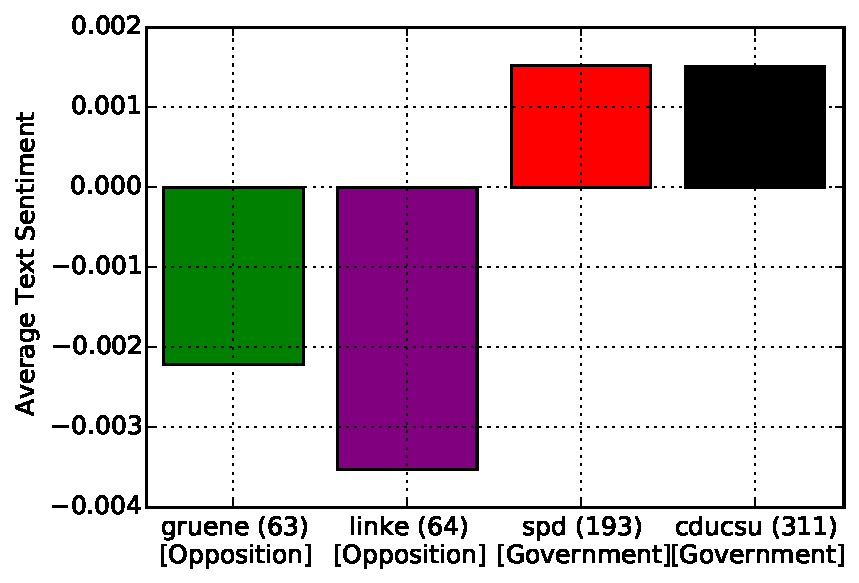
\includegraphics[width=8cm]{images/party-sentiments-18.pdf} 
%
\end{center}
\caption{
\label{fig:party_sentiments}
Speech sentiments computed for speeches of each party (parties are ordered according to political power measured in number of seats in the parliament from left to right). The more political power a party has, the more positive the speech content is, the fewer seats a party has the more words associated with negative emotions are used in a speech. 
}
\end{figure}

\begin{table}[t]
\begin{center}
\begin{tabular}{lrr}
   Sentiment vs. &          Gov. Member    &  Seats\\
\hline\hline
17th period    &  0.84 & 0.70\\
18th period    &  0.98 & 0.89\\
%
\end{tabular}
\end{center}
\caption{
\label{tab:results_avg_political_view}
Correlation coefficient between average sentiment of political speeches of a party in the german bundestag with two measures of their political power, a) their membership in the government and b) with the number of seats that party occupies in the parliament. Shown are correlations for the 17th legislative period and the (ongoing) 18th legislative period.
}
\end{table}



\subsection{Correlations between words and parties}\label{sec:word_party_correlations}

\autoref{fig:party_word_correlations} shows the correlations of individual words and each party. We plotted the top 20 words for each sign, i.e. the 20 words with the strongest positive and negative correlations for each party, respectively. While the correlations do indicate that there are -- despite extensive and careful cleaning procedures -- still words with strong correlations in the top words, we conjecture that at least some of these words do have some discriminatory power, even if they do not refer to political views. Below we list some examples, but the most prominent is probably: the opposition often addresses the government in their speeches, the govermental parties do that less often. This is reflected in the frequency of the usage of words that refer to members of the government or ministers. But among the often used and avoided words we also find words that refer to actual political content. Thus we hypothesize that to some extent these correlation coefficients can give hints as to what the bag-of-words histogram representation into which we transformed the speeches are related to the actual content of the speeches. In the following we give some examples of words that appear to be preferentially used or avoided by each respective party. Even though interpretations of these quantitative results are somewhat invalid, as they neglect the context in which these words were mentioned, we find some interesting patterns. 

\begin{figure}
\begin{center}
%\includegraphics[width=3.5cm]{party_word_correlations-linke.pdf} 
%\includegraphics[width=3.1cm]{party_word_correlations-gruene.pdf} 
%\includegraphics[width=3.45cm]{party_word_correlations-spd.pdf} 
%\includegraphics[width=3.65cm]{party_word_correlations-cdu.pdf}
%
\end{center}
\caption{
\label{fig:party_word_correlations}
Correlations between words and party for parliament speeches. }
\end{figure}


\section{Conclusions and Outlook}\label{sec:conclusion}

%-- in fact even the very definition of a spectrum could be considered a difficult problem. The aim of this study is to investigate


\small
\subsection*{Acknowledgements}

%
\small{
\bibliographystyle{plain}
\bibliography{political_bias_prediction} 
}


\end{document}
